\documentclass[uplatex]{sumiilab-paper}
%% platex を使う場合:
%% \documentclass{sumiilab-paper}

\usepackage[dvipdfmx]{graphicx} % 各種形式の画像を簡単にincludeできます
\usepackage{amsmath,amssymb} % 数式
\usepackage{bm}
\usepackage{mathtools} % 数学記号
\usepackage{cite} % 引用
\usepackage{enumitem} % リスト環境
\usepackage{bussproofs} % 証明器

\usepackage{listings, jvlisting} % ソースコード
\usepackage{amsthm} % 定理環境

%% =========================================
%% 定理環境の設定
%% =========================================
\newtheoremstyle{mystyle}% name
{}% space above
{}% space below
{\normalfont}% body font
{}% indent amount
{\bfseries}% theorem head font
{ }% punctuation after theorem head
{4pt}% space after theorem head (default: 5pt)
{\thmname{#1}\thmnumber{#2}\thmnote{\hspace{2pt}(#3)}}% theorem head spec

\theoremstyle{mystyle}
\newtheorem{definition}{定義}
\newtheorem{theorem}[definition]{定理}
\newtheorem{corollary}[definition]{系}
\newtheorem{proposition}[definition]{命題}
\newtheorem{lemma}[definition]{補題}
\newtheorem{example}[definition]{例}
\newtheorem{assumption}[definition]{仮定}
\newtheorem{axiom}[definition]{公理}
\renewcommand{\proofname}{\bf{証明}}
\numberwithin{definition}{chapter} % 定義1.1のように表示

%% ソースコードのキャプション名
\renewcommand{\lstlistingname}{ソースコード}
%% ===============================================
%% 論文の表紙に表示される情報
%% ===============================================

% 論文の年度と種類
\paper{20XX 年度 卒業論文}% 学部生
%\paper{20XX 年度 修士論文}% 修士

% 論文のタイトル
\title{住井研究室の\\ステキな論文クラスファイルの使用例}

% 学籍番号と著者のお名前
\author{X0XX1234 ラムダ 小太郎}

% 著者の所属
\institute{東北大学 工学部\\電気情報物理工学科}% 学部生
%\institute{東北大学 大学院情報科学研究科\\情報基礎科学専攻}% 修士

% 指導教員のお名前
\supervisor{住井 英二郎 教授}% 指導教員
\subsupervisor{松田 一孝 准教授}% 論文指導教員(省略可)

% 論文発表日時
\date{20XX 年1月1日 \quad 23:00--23:30}
% 発表場所
\venue{電子情報システム・応物系1号館2階トイレ}

%% ===============================================
%% ソースコードの設定
%% ===============================================

% プログラミング言語と表示するフォント等の設定
\lstset{
  language={[Objective]Caml},% プログラミング言語
  basicstyle={\ttfamily\small},% ソースコードのテキストのスタイル
  keywordstyle={\bfseries},% 予約語等のキーワードのスタイル
  commentstyle={},% コメントのスタイル
  stringstyle={},% 文字列のスタイル
  frame=trlb,% ソースコードの枠線の設定 (none だと非表示)
  numbers=left,% 行番号の表示 (none だと非表示)
  numberstyle={\footnotesize},% 行番号のスタイル
  xleftmargin=15pt,% 左余白
  xrightmargin=5pt,% 右余白
  keepspaces=true,% 空白を維持する
  mathescape,% $ で囲った部分を数式として表示する ($ がソースコード中で使えなくなるので注意)
  % 手動強調表示の設定
  moredelim=[is][\bfseries]{@*}{*@},
  moredelim=[is][\itshape]{@/}{/@}
}
\lstMakeShortInline[columns=fullflexible]|% 本文中にコードを|foo|の形式で書くことができます

%% ===============================================
%% 論文中で使う記号とかのマクロ定義
%% ===============================================

%% 論文中で繰り返し使う記号は次のように「マクロ」として実装しておくと良い。
%% TeX ソース中で \BOOL と書くと、\texttt{Bool} に置き換えてくれる。
%% フォントを変え忘れたりするリスクが減るし、あとから記号を変更するのも楽になる。

\newcommand{\bkeyword}[1]{\ensuremath{\mathbf{#1}}}
\newcommand{\BOOL}{\bkeyword{Bool}}
\newcommand{\TRUE}{\bkeyword{true}}
\newcommand{\FALSE}{\bkeyword{false}}
\newcommand{\IF}{\bkeyword{if}}
\newcommand{\THEN}{\bkeyword{then}}
\newcommand{\ELSE}{\bkeyword{else}}

\begin{document}
\frontmatter% ここから前文

\maketitle

\begin{abstract}
ステキな論文の概要
\end{abstract}

\tableofcontents% 目次

\mainmatter% ここから本文

\chapter{序論}

%% 参考文献は \cite{ID} とします(ID は refs.bib 内で文献につけた識別子)
%% BibTeX の使い方などは各自調べて下さい。
序論とか結論とか \cite{Pierce:TypeSystems}

\chapter{\TeX の簡単な使い方}

\section{BNF の書き方の例}

本節では、BNF によるプログラミング言語の構文の書き方を紹介する。
構文木の書き方は一つというわけではないので、幾つかのバリエーションを紹介する。
どの方法が良いと思うかは、個人の好みに依るところなので、好きなものを使えば良いと思う。

まず、次の方法では、array 環境を使って、BNF を書いている。
array 環境は数式環境中で表のようなものを書くときに使う。
基本的に、table 環境と使い方は同じである。
\[
%% 空白を明示的に開けるときは "\," "\ " "~" "\quad" "\qquad" などを使う。
%% 空白の幅は "\qquad" > "\quad" > "~" = "\ " > "\," の順で大きい。
%% "~" と "\ " は空白の代わりに改行を許すかどうかの違い("\ " だと改行される可能性がある)
\begin{array}{rcl@{\qquad\qquad}r}
  t & \Coloneqq & & \text{terms:} \\
  & \mid & x & \text{variables} \\
  & \mid & \lambda x.~t & \text{lambda abstraction} \\
  & \mid & t_1~t_2 & \text{application} \\
  & \mid & \TRUE & \text{true} \\
  & \mid & \FALSE & \text{false} \\
  & \mid & \IF~t_1~\THEN~t_2~\ELSE~t_3 & \text{if statement}
\end{array}
\]

他にも、次のように、align 環境を使っても、似たようなものを書くことができる。
\begin{align}
  t \Coloneqq & \tag*{terms:} \\
  {}\mid{} & x \tag*{variables} \\
  {}\mid{} & \lambda x.~t \tag*{lambda abstraction} \\
  {}\mid{} & t_1~t_2 \tag*{application} \\
  {}\mid{} & \TRUE \tag*{true} \\
  {}\mid{} & \FALSE \tag*{false} \\
  {}\mid{} & \IF~t_1~\THEN~t_2~\ELSE~t_3 \tag*{if statement}
\end{align}
array 環境を愚直に使う場合と比べて、式が中央揃えになるという点と、
``variables'' とかの説明が右端に来ている点が違う。
説明は tag* マクロで出しており、これはもともと式番号を指定するためのものなので、
若干使い方がおかしい気もするが、まぁ、いいだろう。
自分の好みの方を使うと良いだろう。

BNF 全体を左揃えにしたいならば、次のように、flalign 環境を使うと良い。
align 環境と違って、\verb|&| を余分に1つ付ける必要がある、ということに注意して欲しい(詳しくはソースコードを見よ)。
\begin{flalign}
  t \Coloneqq & & \tag*{terms:} \\ % & を余分に1つ付けること!
  {}\mid{} & x \tag*{variables} \\
  {}\mid{} & \lambda x.~t \tag*{lambda abstraction} \\
  {}\mid{} & t_1~t_2 \tag*{application} \\
  {}\mid{} & \TRUE \tag*{true} \\
  {}\mid{} & \FALSE \tag*{false} \\
  {}\mid{} & \IF~t_1~\THEN~t_2~\ELSE~t_3 \tag*{if statement}
\end{flalign}

\section{導出木の書き方の例}

導出木の書き方も色々あるが、ここでは、bussproofs.sty を使った方法を紹介する。
導出木は、手書きでも書きにくいが、\LaTeX だから書きやすいというわけでもなく、
(使うパッケージにも依るが)そこそこの苦労は必要である。
bussproofs.sty を除く多くの方法では、frac などをベースに「分数」で導出木を書く。
bussproofs.sty はこれらとは全く異なるインタフェースであり、慣れれば比較的解りやすい。
bussproofs.sty の動作は、(導出木を要素とする)スタックをイメージすると解りやすい。
よく使うマクロは次の通り。
\begin{itemize}
\item \verb|\AxiomC{...}|:Axiom を push する(導出木では葉に相当)
\item \verb|\UnaryInfC{...}|:スタックから部分導出木(仮定)を1つ pop して、
  それを新たに作ったノード(結論)の子供にすることで、新たな部分導出木を作成し、push する。
\item \verb|\BinaryInfC{...}|:スタックから部分導出木(仮定)を2つ pop して、
  \verb|\UnaryInfC| と同様の動作を行う。
\item \verb|\TrinaryInfC{...}|:スタックから部分導出木(仮定)を3つ pop して、
  \verb|\UnaryInfC| と同様の動作を行う。
\end{itemize}

実際の使い方は以下の通り。

%% T-Var
\begin{prooftree}
  \AxiomC{$x:T \in \Gamma$}
  \RightLabel{\textsc{T-Var}}
  \UnaryInfC{$\Gamma \vdash x : T$}
\end{prooftree}
%% T-Abs
\begin{prooftree}
  \AxiomC{$\Gamma, x:T \vdash t : U$}
  \RightLabel{\textsc{T-Abs}}
  \UnaryInfC{$\Gamma \vdash \lambda x.~t : T \to U$}
\end{prooftree}
%% T-App
\begin{prooftree}
  \AxiomC{$\Gamma \vdash t_1 : T \to U$}
  \AxiomC{$\Gamma \vdash t_2 : T$}
  \RightLabel{\textsc{T-App}}
  \BinaryInfC{$\Gamma \vdash t_1~t_2 : U$}
\end{prooftree}

\begin{prooftree}
  \AxiomC{}
  \RightLabel{\textsc{T-True}}
  \UnaryInfC{$x : \BOOL \to \BOOL \vdash \TRUE : \BOOL$}
  \RightLabel{\textsc{T-Abs}}
  \UnaryInfC{$\vdash \lambda x.~\TRUE : (\BOOL \to \BOOL) \to \BOOL$}
  \AxiomC{$y : \BOOL \in y : \BOOL$}
  \RightLabel{\textsc{T-Var}}
  \UnaryInfC{$y : \BOOL \vdash y : \BOOL$}
  \RightLabel{\textsc{T-Abs}}
  \UnaryInfC{$\vdash \lambda y.~y : \BOOL \to \BOOL$}
  \RightLabel{\textsc{T-App}}
  \BinaryInfC{$\vdash (\lambda x.~\TRUE)~(\lambda y.~y) : \BOOL$}
\end{prooftree}

\section{定理環境}

amsthm.styをカスタマイズした定理環境を使う。

\begin{theorem}[定理のタイトル]
  定理の内容
\end{theorem}

\begin{lemma}[補題のタイトル]
  補題の内容
\end{lemma}

\begin{corollary}[系のタイトル]
  系の内容
\end{corollary}

\begin{proposition}[命題のタイトル]
  命題の内容
\end{proposition}

\begin{definition}[定義のタイトル]
  定義の内容
\end{definition}

\begin{example}[例のタイトル]
  例の内容
\end{example}

\begin{assumption}[仮定のタイトル]
  仮定の内容
\end{assumption}

\begin{axiom}[公理のタイトル]
  公理の内容
\end{axiom}

\begin{proof}
  証明の内容
\end{proof}

\subsection{定理環境の使い方の例}

\begin{lemma}
  \label{lem:interesting-lemma}
  論文の中で最重要とは言えないような性質・命題は補題 (lemma) にする。
  補題や定理から直ちに導けるような軽い命題は系 (corollary) にする(細かい使い分けは人による)。
\end{lemma}

\begin{proof}
  \lstinline|proof*| のように、アスタリスク付きの環境では、番号が付かない。
\end{proof}

\begin{theorem}
  \label{thm:wonderful-theorem}
  提案手法の最も重要な性質や命題は、定理 (theorem) として書く。
  読者の心をくすぐる興味深いステートメントを書こう。
\end{theorem}

\begin{proof}
  定理 \ref{thm:wonderful-theorem} の華麗な証明。その美しい証明に、読者の目は釘付けだ!
  \begin{enumerate}[leftmargin=0pt,itemindent=*,label=Case \arabic*.]
  \item 自明
  \item 補題 \ref{lem:interesting-lemma} から直ちに導ける。
  \item 言うまでもない。目を瞑れば証明が見えてくる。
  \item あんまり自明じゃない
    \begin{enumerate}[label=(\roman*)]
    \item 自明じゃないと思ったけど、やっぱり自明だった
    \item ほらね、こんなに簡単
    \end{enumerate}
  \end{enumerate}
\end{proof}

\section{ソースコード}

ソースコード\ref{src:listup_nodes}は二分木を深さ優先探索して、ノードを列挙する関数である。
\begin{lstlisting}[caption=二分木のノードのリストアップ,label=src:listup_nodes]
type 'a bin_tree =
  | Leaf of 'a
  | Node of 'a bin_tree * 'a bin_tree

let rec listup_nodes = function
  | Leaf x -> [x]
  | Node (r, l) -> (listup_nodes r) @ (listup_nodes l)
\end{lstlisting}

余談ではあるが、こういった参照が飛ばされるような(本文から完全に独立した)ソースコードは図として扱い、キャプションを下につける流儀が一般的かと思う。
というか、そうでない論文を見たことがない。


\section{図}

図の貼り方ぐらいも例はあった方がよいかと(少なくとも本文で最初に言及された場所よりも後ろに配置するのが原則です)。
さすがに PNG 等は |convert| せずに graphicx でそのまま扱う手法を推奨します:図\ref{f:aaa}は dblp\_bibtex\_crossref です。

もし graphicx を持っていない場合は |tlmgr install graphicx| で入るのでは(知らんけど)。
駄目そうならトップの usepackage と本セクションをコメントアウトした本ファイルを origin に |git push| して引き継ぐようにしてください。

\begin{figure}[t]
  \centering
  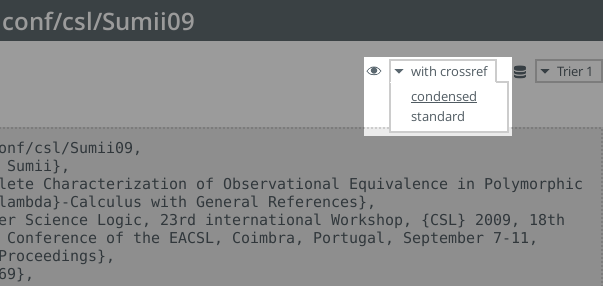
\includegraphics[width=.98\linewidth]{../docs/dblp_bibtex_crossref.png}
\caption{試しに貼り付けられたdblp\_bibtex\_crossref}
\label{f:aaa}
\end{figure}

\chapter{結論}


\backmatter% ここから後付
\chapter{謝辞}

ステキな論文の謝辞

%% 参考文献: bibtex
\bibliographystyle{jplain}
\bibliography{refs}

\appendix% ここから付録
\chapter{ステキな付録}
適当な付録。
\end{document}
